\documentclass[11pt,a4paper]{article}
\usepackage[T1]{fontenc}
\usepackage{mathptmx}
\usepackage[margin=23mm,headheight=15pt]{geometry}
\usepackage{graphicx,xcolor,booktabs,amsmath}
\usepackage{fancyhdr,caption,hyperref}
\definecolor{ink}{HTML}{193B4A}
\definecolor{accent}{HTML}{007C83}
\definecolor{pale}{HTML}{EAF3F4}
\definecolor{muted}{HTML}{52616B}
\hypersetup{colorlinks=true,linkcolor=accent,urlcolor=accent,citecolor=accent,
 pdftitle={Kelani River fish: computational reanalysis of previously reported findings},
 pdfauthor={Tharuniya Anpalakan}}
\graphicspath{{../../figures/}{../../assets/wet_lab/}}
\captionsetup{font=small,labelfont={bf,color=accent},skip=7pt}
\pagestyle{fancy}
\fancyhf{}
\fancyhead[L]{\small\sffamily\color{muted} KELANI RIVER FISH}
\fancyhead[R]{\small\sffamily\color{muted} Computational reanalysis}
\fancyfoot[L]{\footnotesize\color{muted} Aggregate observations \enspace / \enspace Private review edition}
\fancyfoot[R]{\small\thepage}
\renewcommand{\headrulewidth}{0.3pt}
\setlength{\parindent}{0pt}
\setlength{\parskip}{6pt}
\setlength{\emergencystretch}{1.5em}
\renewcommand{\arraystretch}{1.2}
\newcommand{\organism}[1]{\textit{#1} spp.}
\newcommand{\sectiontitle}[1]{\section{\color{ink}#1}}
\newcommand{\photopanel}[3]{\begin{minipage}[t]{0.47\textwidth}\centering
 \includegraphics[width=\linewidth,height=45mm,keepaspectratio]{#1}\par
 \small\textbf{#2}\par #3\end{minipage}}

\begin{document}
\begin{titlepage}
\thispagestyle{empty}
{\sffamily\color{accent}\bfseries RESEARCH PORTFOLIO\quad /\quad COMPUTATIONAL EXTENSION}\par
\vspace{15mm}
{\sffamily\bfseries\color{ink}\Huge Microbiological surveillance\\[3mm]of Kelani River fish}\par
\vspace{8mm}
{\Large Computational reanalysis and visualization of previously reported microbiological findings}\par
\vspace{8mm}
{\color{accent}\rule{\textwidth}{1.2pt}}\par
\vspace{5mm}
\textbf{Prepared by Tharuniya Anpalakan}\par
Computational work assembled on 16 October 2026\par
\vspace{5mm}
\colorbox{pale}{\parbox{\dimexpr\textwidth-2\fboxsep\relax}{\vspace{3mm}
\textbf{27 fish\quad\textbar\quad4 anatomical sites\quad\textbar\quad3 reported organism groups}\par
Source-attributed counts, descriptive comparisons, marginal Wilson intervals and original laboratory evidence.\vspace{3mm}}}
\vfill
\textbf{Original conference research}\par
\emph{Evidence of Foodborne Pathogen Contamination in Riverine Fish from Kelani River, Sri Lanka: A Public Health Perspective}\par
Anpalakan T; Meddage AKMMK\textsuperscript{1,2}; Liyanage GY\textsuperscript{2,3};
Idroos FS\textsuperscript{2}; Manage PM\textsuperscript{2*}.\par
{\small
\textsuperscript{1}Faculty of Graduate Studies, University of Sri Jayewardenepura.\\
\textsuperscript{2}Centre for Water Quality and Algae Research, Department of Zoology, University of Sri Jayewardenepura.\\
\textsuperscript{3}Faculty of Urban Science and Aquatic Bioresources, University of Sri Jayewardenepura.}
\par\vspace{4mm}
\textbf{Printed abstract identifier: PP--137; page 189.}\par
{\small Complete conference venue, year, proceedings metadata and peer-review status remain unverified. The original university report names the Department of Zoology, Faculty of Applied Sciences, University of Sri Jayewardenepura.}\par
\vspace{5mm}
{\small\color{muted} This is a later computational extension, not a new experimental publication. Original photographs are included for private review pending redistribution clearance.}
\end{titlepage}

\sectiontitle{Research context and scope}
\subsection*{Abstract}
Twelve published organism-by-site detection counts from 27 fish were digitized and compared with the university project report. Detection percentages were recalculated and accompanied by two-sided 95\% Wilson score intervals. Reported detection ranged from 55.6 to 100.0\% for \organism{Staphylococcus}, 14.8 to 40.7\% for \organism{Salmonella}, and 18.5 to 55.6\% for \organism{Shigella}. The report discussion contains a conflicting gut denominator and mispaired percentages. The original inferential p-values cannot be validated from marginal counts alone. The extension provides reproducible figures, transparent source reconciliation and a clear boundary between observed detections and biological interpretations.

\subsection*{Research question}
How do the reported detection frequencies vary across skin, mouth, gills and gut, and what conclusions are supported by the available aggregate observations?

\subsection*{Original study and scientific context}
The abstract describes fish obtained through local fishermen across three basin zones and identifies \textit{Oreochromis mossambicus}, \textit{O. niloticus}, \textit{Labeo rohita} and \textit{Heteropneustes fossilis}~\cite{abstract}. The final report gives a different species list; no specimen-level assignments are recoverable. Skin, mouth and gills are exposure interfaces, while gut samples reflect ingestion or residence; these possibilities do not establish a contamination mechanism.

Prior Kelani Basin water research provides environmental context but used different matrices and sampling periods~\cite{kelani}. Culture and biochemical descriptions support presumptive identification; this reanalysis does not independently establish species, virulence or clinical risk. For example, a genus-level \textit{Staphylococcus} finding does not establish the enterotoxin-mediated hazard described for \textit{S. aureus}~\cite{cdc}.

\subsection*{Experimental contribution and personal attribution}
The final report records anatomical sampling, sample preparation, culture, microscopy and biochemical observations~\cite{report}. Tharuniya Anpalakan is the named university candidate and report author. The original abstract has five authors. The documents do not establish who performed each bench step; specific techniques are therefore attributed to the study team. Senior Professor Pathamalal M. Manage is the principal supervisor, and Mr Anjana Kelum is acknowledged for guidance.

\subsection*{Computational objectives}
The new work transcribes aggregate readings with provenance, validates arithmetic, calculates descriptive ranges and marginal uncertainty, reconciles conflicting source values, and generates reproducible figures. It adds no specimens, geospatial coordinates or reconstructed individual outcomes.

\clearpage
\sectiontitle{Data and statistical methods}
The primary analysis uses the twelve counts in the supplied abstract, PDF page 1 / printed page 189. Report results on pages 15--16 repeat those counts. A separate source reading retains the conflicting \(22/25\) denominator on report page 20. Each CSV row includes the organism group, site, integer numerator and denominator, source document, page, section and verification status.

For a positive count \(x\) among \(n\) specimens, the detection estimate is \(\widehat p=x/n\). Its percentage is \(100\widehat p\). The Wilson score limits are
\begin{equation}
\frac{\widehat p+z^2/(2n)\;\pm\;z\sqrt{\widehat p(1-\widehat p)/n+z^2/(4n^2)}}{1+z^2/n},
\qquad z=\Phi^{-1}(0.975).
\end{equation}
The implementation handles the boundary cases \(x=0\) and \(x=n\). A 100\% observed detection proportion has a lower uncertainty limit below 100\%.

\textbf{Interpretation of intervals.} These are descriptive marginal intervals for one organism-site proportion, conditional on independent, comparable fish-level observations. They are not intervals for paired site contrasts, simultaneous confidence bands, or design-adjusted estimates for the full river basin. Repeated anatomical sites on each fish share a sampling unit.

\par
\begin{table}[ht]
\centering\small
\caption{Published counts, recalculated detection percentages and marginal 95\% Wilson intervals. Values are generated directly from the validated abstract rows.}
\label{tab:counts}
% Generated by scripts/build_latex_report.py; do not edit by hand.
\begin{tabular}{llrrr}
\toprule
Reported group & Site & Positive/total & Detection (\%) & 95\% Wilson CI (\%) \\
\midrule
\textit{Staphylococcus} spp. & Skin & 27/27 & 100.0 & 87.5--100.0 \\
 & Mouth & 27/27 & 100.0 & 87.5--100.0 \\
 & Gills & 15/27 & 55.6 & 37.3--72.4 \\
 & Gut & 22/27 & 81.5 & 63.3--91.8 \\
\addlinespace
\textit{Salmonella} spp. & Skin & 11/27 & 40.7 & 24.5--59.3 \\
 & Mouth & 9/27 & 33.3 & 18.6--52.2 \\
 & Gills & 10/27 & 37.0 & 21.5--55.8 \\
 & Gut & 4/27 & 14.8 & 5.9--32.5 \\
\addlinespace
\textit{Shigella} spp. & Skin & 9/27 & 33.3 & 18.6--52.2 \\
 & Mouth & 15/27 & 55.6 & 37.3--72.4 \\
 & Gills & 11/27 & 40.7 & 24.5--59.3 \\
 & Gut & 5/27 & 18.5 & 8.2--36.7 \\
\bottomrule
\end{tabular}

\end{table}
\par

The data do not include linked binary outcomes for individual fish. Cochran's Q, McNemar tests and clustered models cannot be reconstructed reliably from these margins. The abstract reports \(p<0.001\) for \textit{Staphylococcus}, \(p=0.17\) for \textit{Salmonella}, and \(p=0.041\) for \textit{Shigella}; these values are quoted as published, without a claim of reproduction. No new confirmatory p-values are calculated.

\clearpage
\sectiontitle{Reported detection patterns}
The largest observed site range is 44.4 percentage points for \textit{Staphylococcus}, followed by 37.0 for \textit{Shigella} and 25.9 for \textit{Salmonella}. These are descriptive differences between marginal percentages; they do not estimate bacterial concentration.
\par
\begin{figure}[ht]
\centering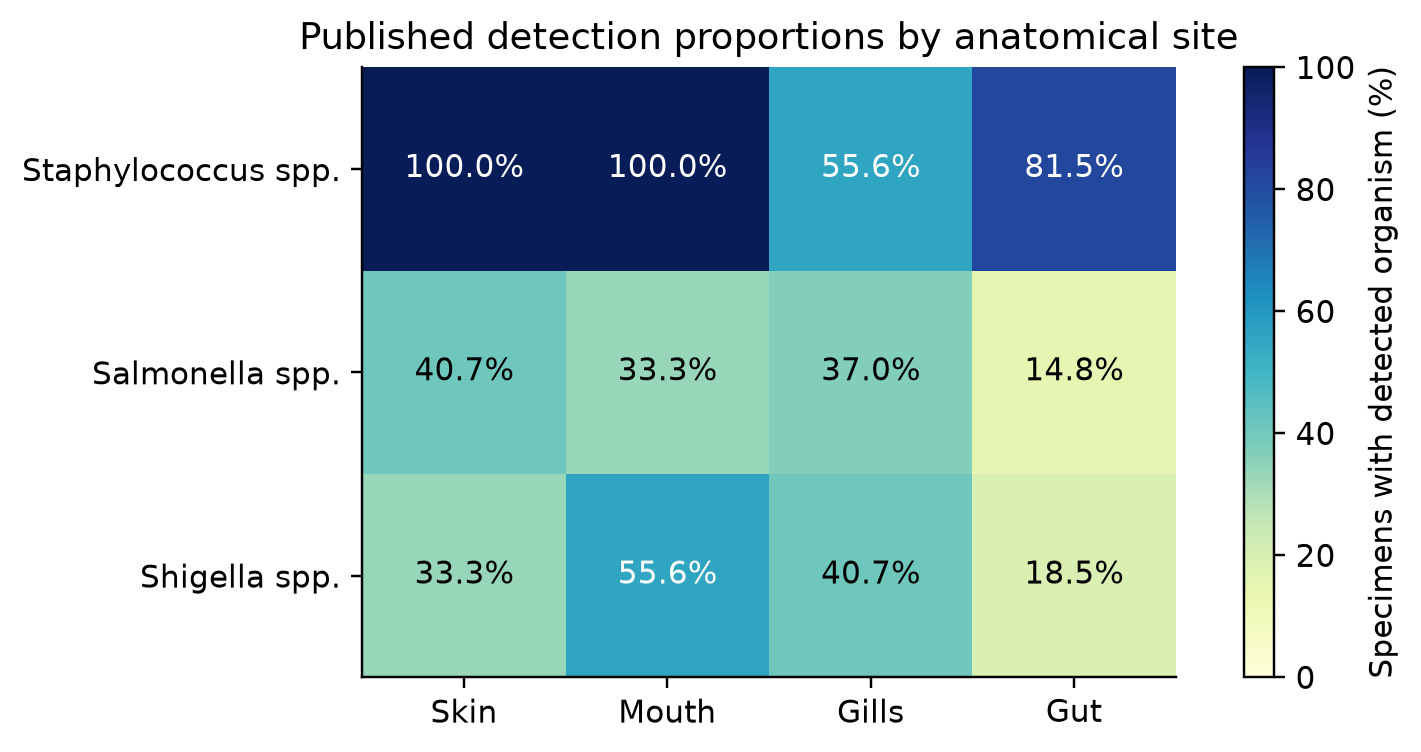
\includegraphics[width=0.94\textwidth]{01_heatmap.png}
\caption{Published organism-by-site detection heatmap. Each cell is \(100x/27\), rounded to one decimal. Source: abstract PP--137, printed p189; report pp15--16 agrees on all counts.}
\end{figure}
\par
\par
\begin{figure}[ht]
\centering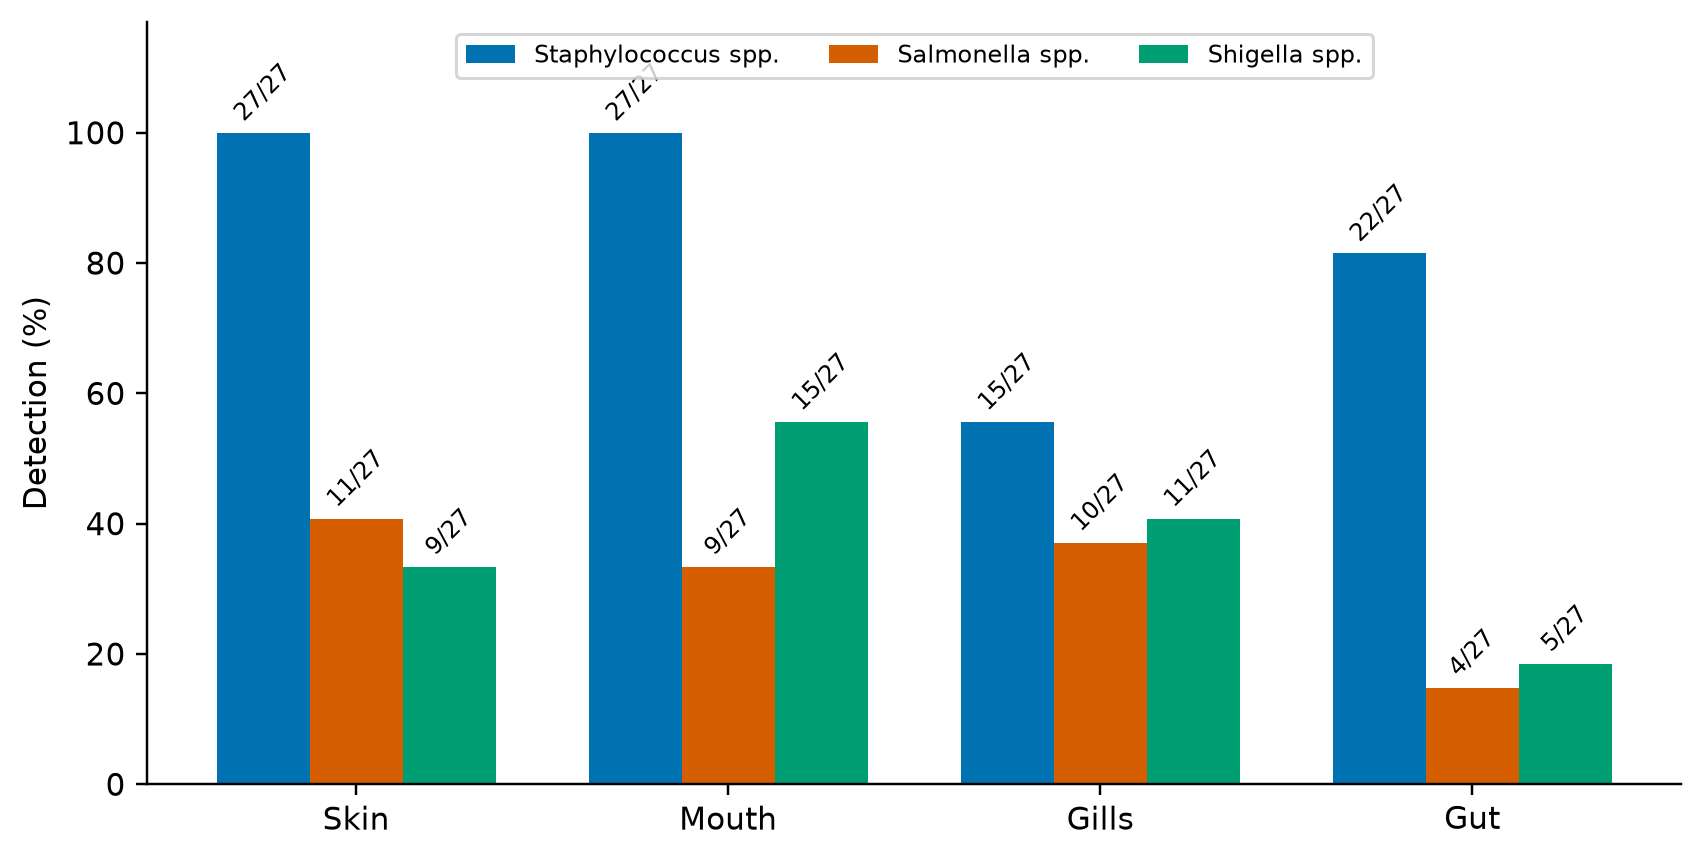
\includegraphics[width=0.94\textwidth]{02_grouped_bars.png}
\caption{Detection percentages with exact numerator/denominator labels. Heights describe positive observations out of 27 fish at each site; they do not represent bacterial load. Source and calculation as in Figure 1.}
\end{figure}
\par

\clearpage
\sectiontitle{Uncertainty and anatomical profiles}
The figures show uncertainty and site patterns separately. Categorical anatomical sites have no assumed numeric distance or continuous order. A difference in marginal point estimates does not by itself establish a statistically supported paired contrast.
\par
\begin{figure}[ht]
\centering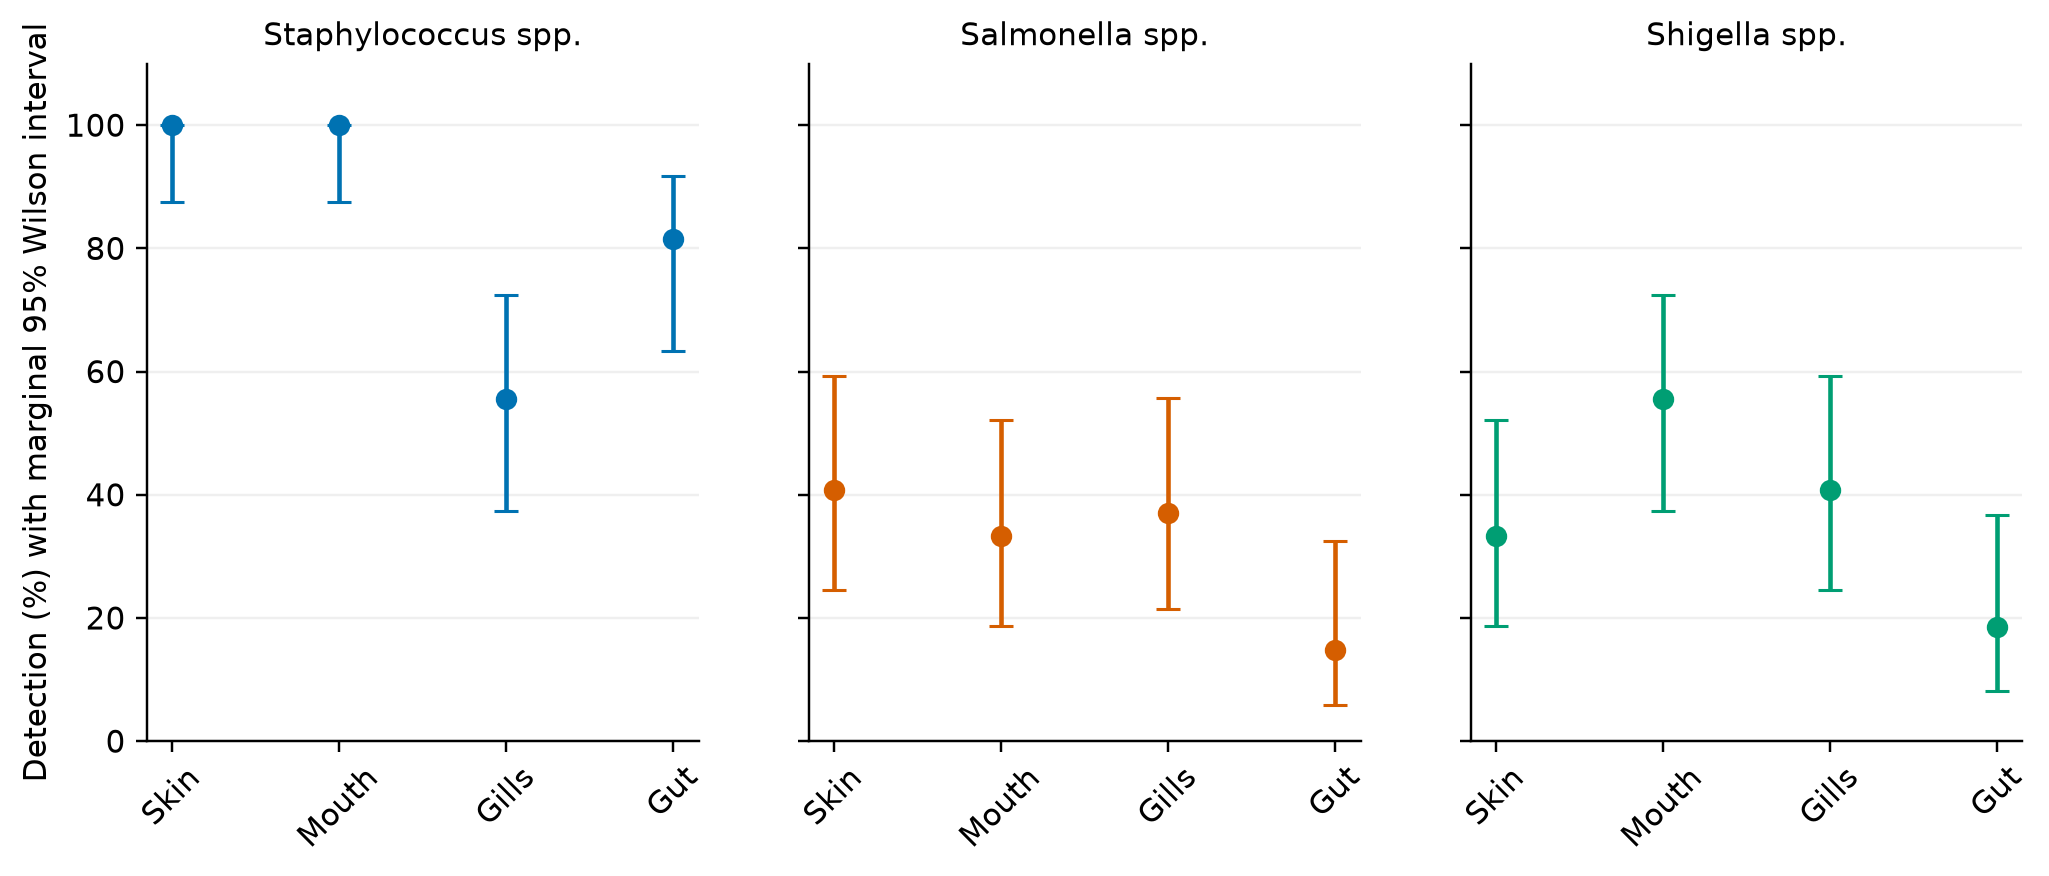
\includegraphics[width=\textwidth]{03_wilson_intervals.png}
\caption{Marginal 95\% Wilson score intervals calculated from the twelve published counts. Whiskers quantify single-proportion binomial uncertainty under the stated assumptions; they do not account for paired site comparisons or basin-zone clustering.}
\end{figure}
\par
\par
\begin{figure}[ht]
\centering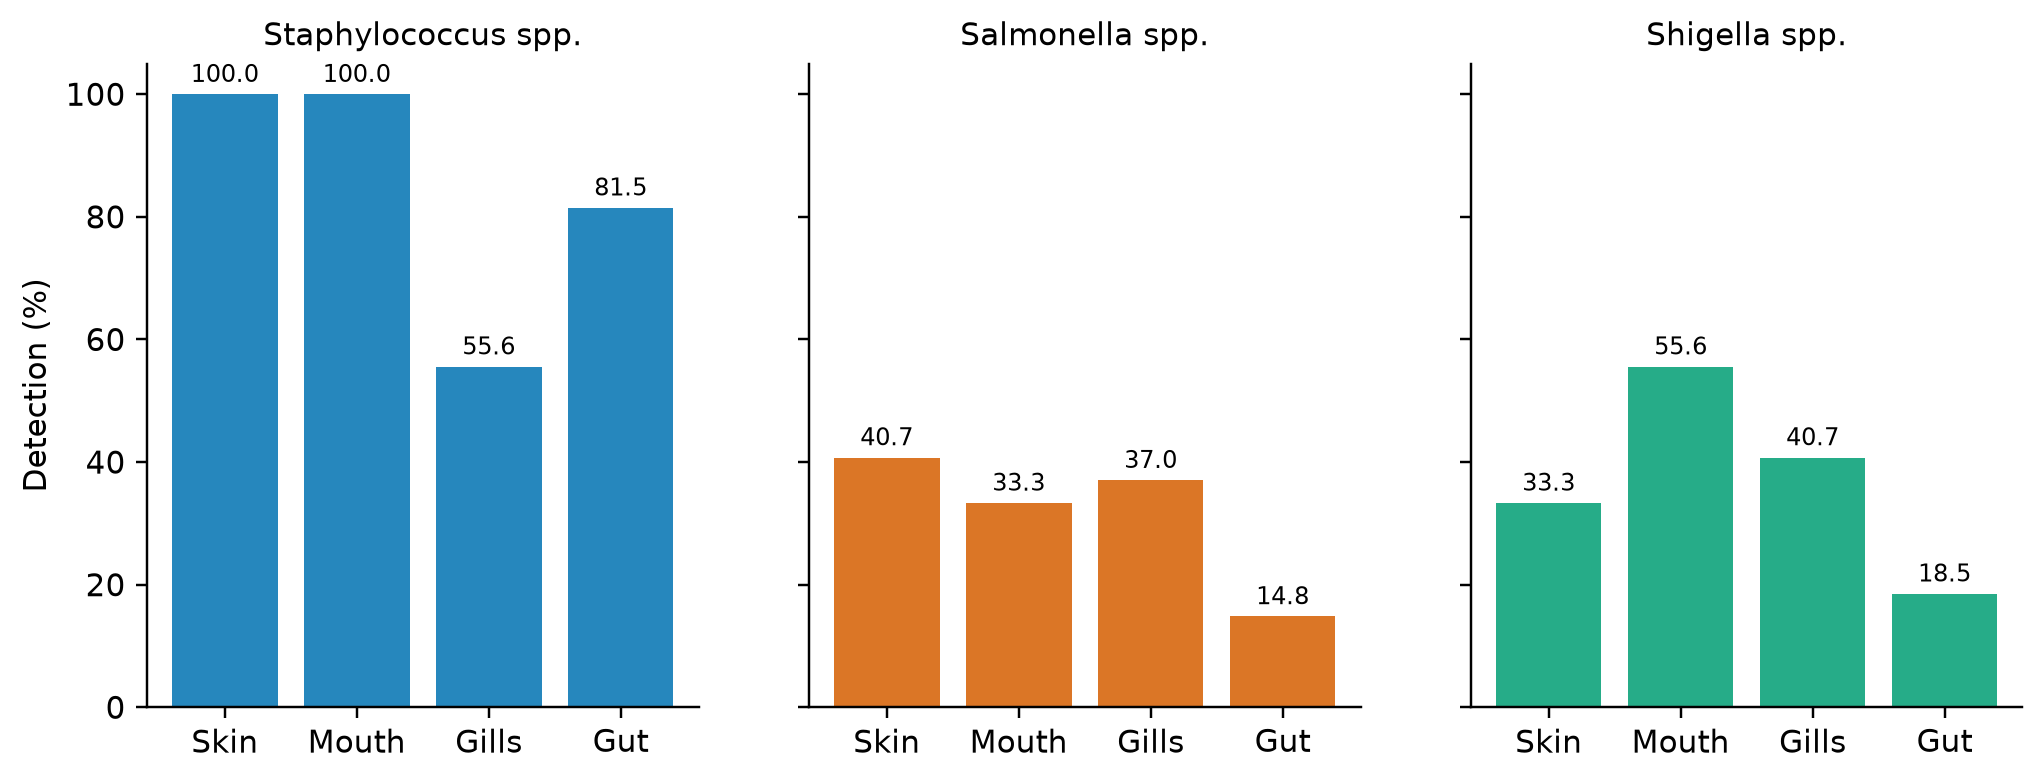
\includegraphics[width=\textwidth]{04_detection_profiles.png}
\caption{Separate anatomical-site profiles for each reported organism group. Bars use \(100x/27\); sites are displayed as discrete categories. Source: abstract PP--137, printed p189.}
\end{figure}
\par
The gut detection proportion for \textit{Staphylococcus} exceeds its gill proportion. Thus a blanket claim that every external site exceeds every internal site is not supported by the published margins. The observations alone also cannot separate environmental exposure, handling contamination and persistent colonization.

\clearpage
\sectiontitle{Workflow, provenance and sensitivity}
\par
\begin{figure}[ht]
\centering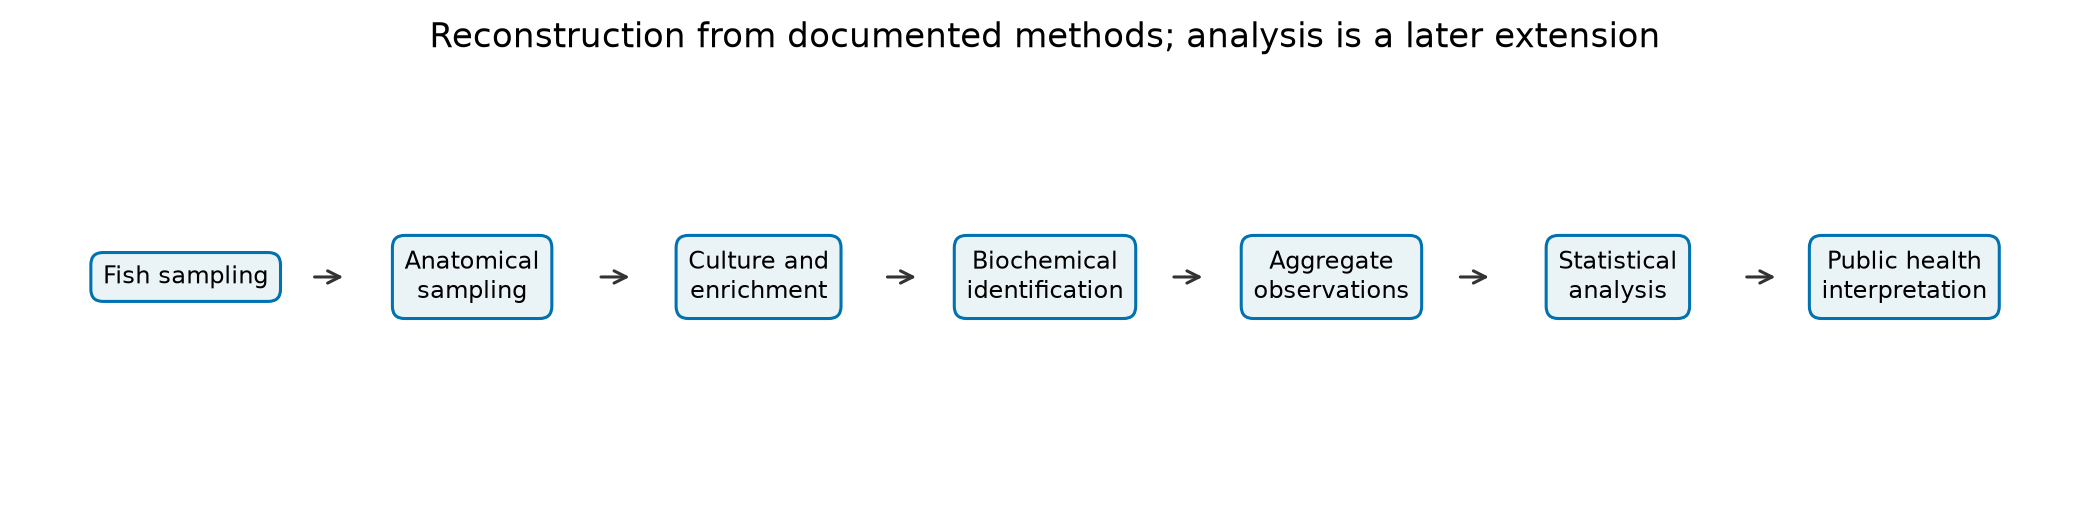
\includegraphics[width=\textwidth]{05_workflow.png}
\caption{High-level reconstruction from the original report p13 and abstract p189. The new statistical analysis and reproducible outputs are computational additions to previously reported experimental observations.}
\end{figure}
\par
\par
\begin{figure}[ht]
\centering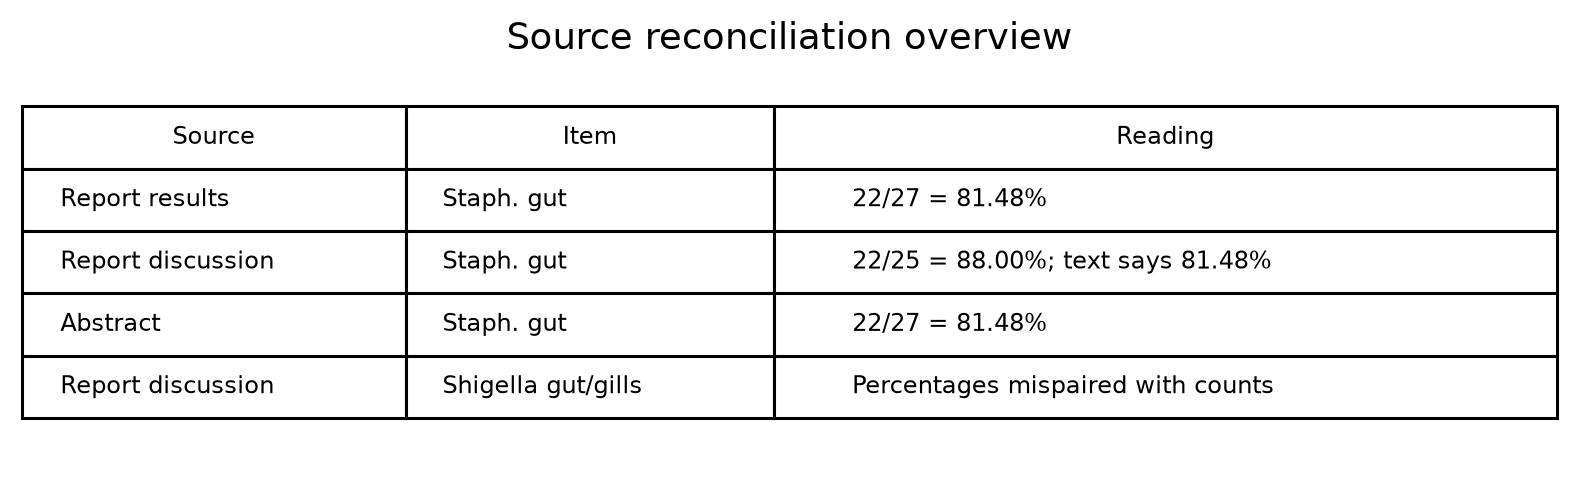
\includegraphics[width=\textwidth]{06_source_comparison.png}
\caption{Source discrepancies retained explicitly: report results p15 versus discussion p20 for the \textit{Staphylococcus} gut denominator, and discussion p21 for the \textit{Shigella} count-percentage pairings.}
\end{figure}
\par
\par
\begin{table}[ht]
\centering\small
\caption{Literal denominator sensitivity for the reported \textit{Staphylococcus} gut count. Both readings are preserved; the abstract reading drives the primary analysis.}
\begin{tabular}{lrrr}
\toprule
Source reading & Fraction & Detection (\%) & 95\% Wilson CI (\%) \\
\midrule
Abstract / report results & 22/27 & 81.48 & 63.30--91.82 \\
Report discussion (literal) & 22/25 & 88.00 & 70.04--95.83 \\
\bottomrule
\end{tabular}

\end{table}
\par
The alternative \(22/25\) equals 88.00\%, whereas \(22/27\) equals 81.48\%: a 6.52 percentage-point difference. The report prints 81.48\% beside \(22/25\), indicating an internal arithmetic inconsistency. The available documents cannot establish why 25 appears or whether specimens were excluded. The \textit{Shigella} discussion mispairs gut and gill percentages, while its results section agrees with the abstract's counts.

\clearpage
\sectiontitle{Original laboratory evidence}
The photographs below were extracted as embedded image bytes from the university report, without altering the source pixels. They illustrate documented laboratory observations and are included for private review pending redistribution permission. Figure numbers inside each panel refer to the original report.
\par
\begin{figure}[ht]
\centering
\photopanel{report_p14_fig02.jpeg}{Culture observation}{Report p14, Fig. 2: mannitol salt agar after incubation in the presumptive \textit{Staphylococcus} workflow.}
\hfill
\photopanel{report_p17_fig13.jpeg}{Microscopy}{Report p17, Fig. 13: microscopic field of a suspected \textit{Staphylococcus} isolate.}
\par\vspace{8mm}
\photopanel{report_p14_fig04.jpeg}{Culture observation}{Report p14, Fig. 4: Salmonella-Shigella agar after incubation in the presumptive \textit{Salmonella} workflow.}
\hfill
\photopanel{report_p18_fig27.jpeg}{Biochemical observation}{Report p18, Fig. 27: Kligler iron agar after incubation in the presumptive \textit{Salmonella} workflow.}
\caption{Selected authentic figures from Tharuniya Anpalakan's university project report, credited to the original study team. They do not independently establish the operator of each procedure, species identity or virulence. The repository image inventory records source pages, captions and rights status.}
\end{figure}
\par
The PDFs contain no field-collection or fish-anatomical-sampling photographs. No generated or stock imagery is used to fill these gaps. The full local image inventory comprises 31 extracted laboratory photographs; eight selections are tracked in the private repository for its README gallery.

\clearpage
\sectiontitle{Discussion and conclusions}
The reanalysis preserves the twelve published aggregate observations and provides an auditable path from counts to tables, intervals and figures. The strongest supported conclusion is that reported detection frequencies differed descriptively among the sampled anatomical sites. Their magnitude, uncertainty and source inconsistencies can be inspected without claiming new experimental findings.

\subsection*{Limits to biological interpretation}
Reported genus-level culture and biochemical findings remain presumptive in this computational work. No independent molecular or serological confirmation, virulence characterization, bacterial concentration or human illness outcome was supplied. A food-safety interpretation therefore requires care: detection does not directly measure infection risk, prove a pollution source or establish persistent fish colonization. External identification guidance illustrates the distinction between presumptive findings and further confirmation~\cite{fda}.

\subsection*{Limits to statistical interpretation}
Linked specimen records, zone assignments, species assignments and the original statistical test are missing. Marginal counts cannot reveal within-fish concordance. Small sample size, an uncertain sampling frame and possible spatial clustering constrain extrapolation. The Wilson intervals do not remedy these design limitations, and overlapping or non-overlapping marginal intervals are not used as tests of paired site effects.

\subsection*{Useful next evidence}
Authenticated specimen-level records would permit verification of denominators and specimen inclusion, reconciliation of species lists, and assessment of an appropriate paired or clustered model. Complete conference bibliographic information and confirmation of individual laboratory roles would improve attribution. These are evidence requirements, not data inferred by the current pipeline.

\subsection*{Conclusion}
The computational extension improves transparency of previously reported findings through explicit provenance, reproducible calculations and scientifically bounded interpretation. It supports a research portfolio connecting experimental microbiology with Python analysis while preserving the original study's authorship and institutional context.

\subsection*{Acknowledgements and disclosure}
Credit is retained for the original five conference authors, Senior Professor Pathamalal M. Manage, Mr Anjana Kelum, the Department of Zoology, Faculty of Applied Sciences, and the Centre for Water Quality and Algae Research, University of Sri Jayewardenepura. AI assistance supported code and editorial preparation. Original photographs and PDFs are outside the software license. Git author and committer timestamps were manually assigned to 25 September 2025 at the owner's request; this report and computational work were assembled in October 2026. Those assigned timestamps do not establish an earlier research or software event.

\clearpage
\sectiontitle{References and reproducibility}
\begingroup\small
\renewcommand{\refname}{Sources}
\begin{thebibliography}{9}
\bibitem{abstract} Anpalakan T; Meddage AKMMK; Liyanage GY; Idroos FS; Manage PM.
\emph{Evidence of Foodborne Pathogen Contamination in Riverine Fish from Kelani River, Sri Lanka: A Public Health Perspective.} Supplied conference abstract, PP--137, printed p189. Full venue and publication year unverified.
\bibitem{report} Anpalakan T. University research project report on bacterial detections in Kelani River fish. Cover submission date: 15 November 2025. Supplied original PDF, 33 pages.
\bibitem{kelani} Mahagamage MGYL, Pathirage MVSC, Manage PM. Contamination Status of Salmonella spp., Shigella spp. and Campylobacter spp. in Surface and Groundwater of the Kelani River Basin, Sri Lanka. \emph{Water}. 2020;12(8):2187. \href{https://doi.org/10.3390/w12082187}{doi:10.3390/w12082187}.
\bibitem{cdc} Centers for Disease Control and Prevention. About Staph Food Poisoning. \url{https://www.cdc.gov/staph-food-poisoning/about/}. Accessed 16 October 2026.
\bibitem{fda} U.S. Food and Drug Administration. Bacteriological Analytical Manual, Chapter 5: Salmonella. \url{https://www.fda.gov/food/laboratory-methods-food/bam-chapter-5-salmonella}. Accessed 16 October 2026.
\end{thebibliography}
\endgroup

\subsection*{Build this manuscript}
The editable source is \texttt{reports/latex/computational\_reanalysis.tex}. Generated tables are calculated by the same Python interval module used by the notebooks; no table estimates are entered manually. Install the pinned Python dependencies and a TeX distribution providing \texttt{pdflatex}, then run from the repository root:
\begin{verbatim}
python -m scripts.build_data
python -m pytest -q
python -m scripts.build_latex_report
\end{verbatim}
The build generates tables, refreshes the six computational figures, runs LaTeX twice and checks for overflowing boxes, missing characters and unresolved references. It exports the manuscript PDF and a machine-readable table of the twelve published estimates and interval bounds. The original source PDFs are needed for source auditing, not for rebuilding the report from the repository's transcription.
\end{document}
